\documentclass[12pt, a4paper]{article}
\usepackage{amsmath}
\usepackage{amsfonts}
\usepackage{amsthm}
\usepackage{mathtools}
\usepackage{tikz}
\usetikzlibrary{bayesnet}
\newtheorem{theorem}{Theorem}[section]
\newtheorem{definition}{Definition}[section]
\numberwithin{equation}{section}
\usepackage{pgfplots}
\pgfplotsset{width=10cm,compat=1.9}
\graphicspath{ {img/} }
\DeclareGraphicsExtensions{.png}

\title{Process Mining}
\author{Kristian Wichmann}

\begin{document}
\maketitle

\section{What is process mining?}
\textit{Process mining} is about discovering underlying procedures and causal relations in data. There is a multitude of models and algorithms that can be used for this. A number of these will be outlined here.

Process mining activities can be divided into three different "modes":

\begin{itemize}
\item \textit{Play-in} is the term we use for the act of taking data and turning it into a process model.
\item In \textit{play-out} we take a process model and examine what kinds of behaviour it allows. This can be done through simulation.
\item \textit{Replay} is the most important part of process mining. Here, modelled and observed behaviours are compared. This is useful for (among other things) conformance checking, prediction, and bottleneck analysis.
\end{itemize}

\section{Event logs}
An \textit{event log} is a common way to represent the raw data used in process mining. The term refers to a collection of data where each row contains at least the following:
\begin{itemize}
\item A \textit{case id} corresponding to a particular unit whose processes we wish to discover.
\item An \textit{activity name}, to denote a specific kind of activity.
\item A \textit{timestamp}, which allows us to order the events.
\end{itemize}
The data may contain other columns (and these may be used in various ways as well), but this is the minimum.

\subsection{Traces of activities}
For each unique case id, we can look at the subset of the event log which matches it. This may then be sorted by the timestamp (if this is not already the case). This will yield a number of strings of activities known as \textit{traces}. Examples of traces could be:
\begin{equation}
\langle abcd\rangle\quad\langle aaacccd\rangle\quad\langle ababababd\rangle
\end{equation}

\section{Model: Petri nets}

\subsection{Petri net graphs}
A \textit{Petri net graph} is a tuple $(P, T, F)$. Here $P$ is a collection of \textit{places} and $T$ a collection of \textit{transitions}, $P$ and $T$ disjoint. The \textit{flow relations} $F\subseteq(P\times T)\cup(T\times P)$ corresponds to place inputs ($I\subseteq P\times T$) and outputs ($O\subseteq T\times P$) to transitions.

\begin{figure}
\centering
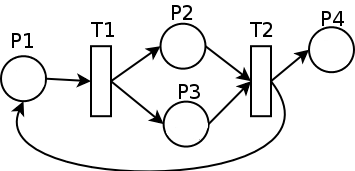
\includegraphics[width=0.7\textwidth]{petri_graph}
\caption{An example of a Petri net graph.}
\label{fig:petri_graph}
\end{figure}

The graphical representation of a petri net graph is to draw places as circles, transitions as thick lines or squares, and flow relations as arrows from places to transitions. As an example, figure \ref{fig:petri_graph} is the graphical representation of the following Petri net graph:
\begin{itemize}
\item $P=\{P1, P2, P3, P4\}$
\item $T=\{T_1, T_2\}$
\item $F=I\cup O$, where:
\begin{align}
I=&\{\{P1, T1\}, \{P2, T2\}, \{P3, T2\}\}\\
O=&\{\{T1, P2\}, \{T1, P3\}, \{T2, P1\}, \{T2, P4\}\}
\end{align}
\end{itemize}

Sometimes, we may wish to allow more than one arrow between a place-transition/transition-place pair. In this case, $F$ instead becomes a function:
\begin{equation}
F: (P\times T)\cup(T\times P)\rightarrow\mathbb{N}_0
\end{equation}
The value of a pair is then the number of arrows. Again, this could be split into input and output functions:
\begin{equation}
I: P\times T\rightarrow\mathbb{N}_0,\quad
O: T\times P\rightarrow\mathbb{N}_0
\end{equation}

\subsection{Markings and Petri nets}

\begin{figure}
\centering
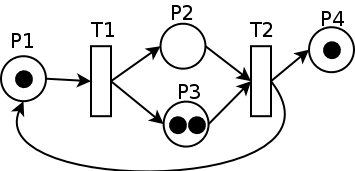
\includegraphics[width=0.7\textwidth]{petri_marking}
\caption{An example of a Petri net.}
\label{fig:petri_marking}
\end{figure}

A \textit{marking} $M$ on a Petri net graph, is a function:
\begin{equation}
M: P\rightarrow\mathbb{N}_0
\end{equation}
This is interpreted as the number of \textit{tokens} present at each place in the Petri net graph. For instance, figure \ref{fig:petri_marking} shows the following marking on the example Petri net graph from the section above:
\begin{equation}
P1\mapsto 1,\quad P2\mapsto 0,\quad P3\mapsto 2,\quad P4\mapsto 1
\end{equation}

A collection of a Petri net graph $(P, T, F)$ and an initial marking $M_0$ on it is called a \textit{Petri net}.

\subsection{Rules of the "game"}
From the initial marking, a Petri net can undergo the transitions in $T$ under certain circumstances.

A transition $t\in T$ is \textit{enabled}, if all the places which has an input flow relation pointing to it all has at least one token\footnote{If several arrows are allowed, each place has to hold at least a number of tokens corresponding to the number or arrows.}.

An enabled transition may \textit{fire}, which means that the current marking changes, such that each token from the input places are removed, while all the output places gets a token\footnote{Again, if several arrows are allowed, several tokens are removed/added according to the multiplicity of arrows.}.

Transitions always happens in a specific order, so two transitions cannot fire at the same time. This means that we may write a \textit{trajectory} of the Petri net as:
\begin{equation}
M_0, M_1, M_2, \ldots,\quad \langle t_1,t_2,\cdots\rangle
\end{equation}
Here, all the $M_i$'s are markings, and between $M_i$ and $M_{i+1}$ transition $t_{i+1}$ fires. Such a trajectory may or may not be finite in length.

The set of all markings that are \textit{reachable} for a Petri net $N$ is denoted $R(N)$. The elements of $R(N)$ forms a directed \textit{reachability graph}, with transitions as edges.

\subsection{Properties of Petri nets}
A marking where no transitions are enable is called \textit{deadlocked}. A Petri net with a deadlocked marking in its reachability graph is said to have a \textit{potential deadlock}.

A transition in a Petri net that can never fire, i.e. is not an edge anywhere in the reachability graph is called \textit{dead} or $L_0$-\textit{live} (a designation that will become clear in a while). A transition that is not dead has some degree of being alive, as shown below:
\begin{itemize}
\item A transition is $L_1$-\textit{live} if it is not dead, i.e. if is occurs as an edge somewhere in the reachability graph. This is also called \textbf{potentially fireable}.
\item  A transition is $L_2$-\textit{live} if for any positive integer $k$ there is a reachable marking in which it occurs at least $k$ times on a trajectory to the marking. (The trajectories can be different for each $k$).
\item  A transition is $L_3$-\textit{live} if there is a trajectory in which the transition occurs infinitely often.
\item  A transition is $L_4$-\textit{live} - or simply \textit{live}, if for any reachable marking, the transition is $L_1$-live. I.e. no matter where in the reachability graph we are, it is always possible to fire the transition some time in the future.
\end{itemize}
These conditions are progressively stronger, so usually only the highest index is used to refer to a given transition.

A place $p$ in a Petri net is called $k$-\textit{bounded} if all markings in the reachability graph has as most $k$ tokens on it. A place that is 1-bounded is called \textit{safe}. A place that is $k$-bounded for any positive value of $k$ is called \textit{bounded}.

A Petri net in which all places are ($k$-)bounded is called  ($k$-)\textit{bounded}. A Petri net in which all places are safe is called \textit{safe}. A Petri net graph in which all possible initial markings are bounded is called \textit{structurally bounded}.

\subsection{Workflow nets}
A \textit{workflow net} (or WF-net for short) is a special kind of Petri net. It is used to model processes with transitions representing events.

A workflow net has a start or \textit{source} place and an ending or \textit{sink} place, so that the source has no inputs, and the sink no outputs. In addition, all other places should be on a trace from the source to the sink. The initial marking is one token at the source.

A workflow net is called \textit{sound} if the following four criteria are satisfied:
\begin{enumerate}
\item Safeness: The WF-net is safe.
\item Proper completion: When a token is placed on the sink, all other places should be empty.
\item Option to complete: It is always possible to eventually get a token to the sink.
\item Absence of dead parts: All transitions are $L_1$-live.
\end{enumerate}
Actually, this is somewhat redundant: Criterium 1 and 3 implies criterum 2:

\begin{theorem}
For a safe workflow net, if there is option to complete, proper completion is also true.
\end{theorem}
\begin{proof}
The statement can be written as $(3)\Rightarrow(2)$. This is equivalent to $\neg (2)\Rightarrow\neg (3)$. So assume that proper completion does not hold. I.e. there is a reachable marking with a token at the end place and at least one other place. But because any place in a WF-net is part of a trace from source to sink, we can eventually move that token to the sink. But this contradicts soundness. So completion is not possible.
\end{proof}

\begin{figure}
\centering
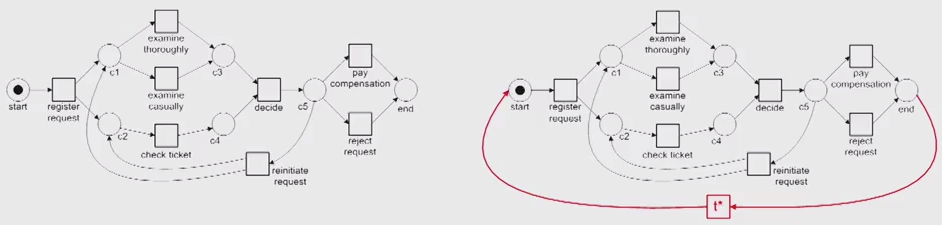
\includegraphics[width=0.9\textwidth]{wf_theorem}
\caption{Adding the transition $t^*$.}
\label{fig:wf_theorem}
\end{figure}

It turns out that there's a connection between sound workflow nets and a specific modification to the net: Given a workflow net, the so-called \textit{short-circuited} Petri net is constructed by adding another transition $t^*$ from the sink to the source. Figure \ref{fig:wf_theorem} shows this process.

\begin{theorem}
A workflow net is sound if and only if the corresponding short-circuited Petri net is live and bounded.
\end{theorem}
\begin{proof}
There's two directions to show. (Coming later)
\end{proof}

\section{The alpha algorithm}

\section{Model: Dependency graph}
A \textit{dependency graph} is a series of nodes - representing events - in which there are causal arrows between events. So as such, this is simply a directed graph.

Because such a graph does not contain any information about splits and joins, it is usually not used as is. Instead it is the basis for more complicated models.

\section{Heuristics mining}



\section{Model: Causal nets}

\end{document}